\section{The Klobuchar ionospheric model}
\label{app:klobuchar}
Given the user position in geodetic latitude $\phi_u$, longitude $\lambda_u$, elevation angle E and azimuth A of the observed satellite, as well as model parameters $\alpha_n$ and $\beta_n$ received from the almanac, the Klobuchar model computes the ionospheric delay $I_{GPS}$ as follows.
\begin{subequations}
\begin{align}
	\psi &= \frac{0.0137}{E + 0.11} - 0.022\\
    \phi_I &= \phi_u + \psi A\\
    \intertext{if $\phi_I > +0.416$, then $\phi_I = +0.416$}
    \intertext{if $\phi_I < -0.416$, then $\phi_I = -0.416$}
    \lambda_I &= \lambda_u + \frac{\psi sin(A)}{cos(\phi_I)}\\
    \phi_m &= \phi_I + 0.064 cos(\lambda_I - 1.617)\\
    t &= 43200\lambda_I + t_{GPS}\\
    \intertext{Where $0 \leq t \leq 86400$. Therefore, if $t \geq 86400$, subtract 86400, if $t < 0$ add 86400}
    A_I &= \sum_{n=0}^{3}\alpha_n\phi_m^n\\
    \intertext{if $A_I < 0$, then $A_I = 0$}
    P_I &= \sum_{n=0}^{3}\beta_n\phi_m^n\\
    \intertext{if $P_I < 72000$, then $P_I = 72000$}
    X_I &= \frac{2\pi(t-50400}{P_I}\\
    F &= 1.0 + 16.0(0.53-E)^3\\
    I_{GPS} &= 
     \begin{cases}
     	(5*10^{-9} + \sum_{n=0}^{3}\alpha_n\phi_m^n)\bigg(1-\frac{X_I^2}{2} + \frac{X_I^4}{24}\bigg)F&\quad, |X_i| \leq 1.57\\
        5*10^{-9}F&\quad, |X_i| \geq 1.57
     \end{cases}
\end{align}


\section{Saastamoinen tropospheric model}
\label{app:saas}
Given the user position in geodetic latitude $\phi_u$, longitude $\lambda_u$, height h, elevation angle E, humidity \textit{hr} and temperature T (in Kelvin). The tropospheric error, $\delta_t$ calculated by the Saastamoinen model is
\begin{subequations}
\begin{align}
	\intertext{if $h < -100$ or $h > 10^4$, $\delta_t = 0$}
    p &= 1013.25(1-2.2557e^{-5})^{5.2568}\\
    e &= 6.108hr\exp^\frac{17.15T-4684}{T-38.45}\\
    z &= \frac{\pi}{2.0}-E\\
    t_{dry} &= \bigg(\frac{0.0022768p}{1-0.00266cos(2\phi_u)}-0.00028h10^{-3}\bigg)/cos(z)\\
    t_{wet} &= \frac{2.857635e}{(T+0.05)cos(z)}\\
    \delta_t &= t_{dry} + t_{wet}
\end{align}
\end{subequations}

\end{subequations}
\begin{figure}[!htbp]
    \centering
    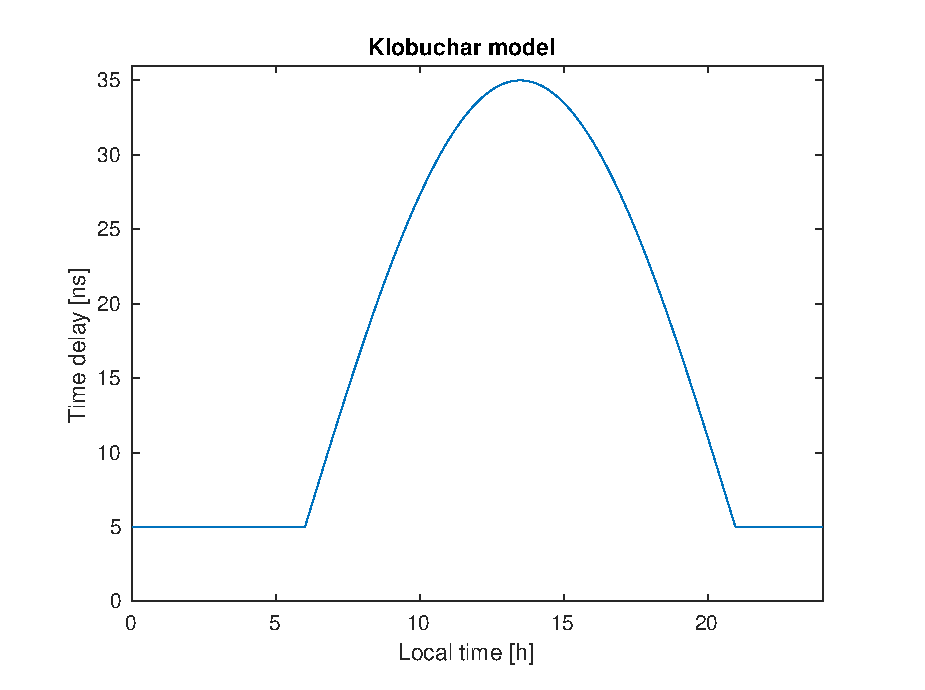
\includegraphics[scale=0.7]{Appendices/bilder/klobuchar.eps}
    \caption{This figure shows the concept of the klobuchar model. Note that this is not exact, but rather a simple approximation to show the concept of the model.}
    \label{fig:klobuchar}
\end{figure}
